\documentclass{article}
\usepackage{graphicx}

\begin{document}

\begin{titlepage}
\title{ECS189G Homework 2 Report Problem A}
\author{Goh Chang Kang, Charles 916751838, \\
Yang Minxing 916751773, Chen Jieyi Chloe 999823783}

\date{October 30, 2018}
\maketitle
\end{titlepage}


\section{Problem A}
We begin by loading the relevant datasets, libraries (rectools and recosystem) and splitting the dataset into test set and training set. For the test set we decided to use 1000 entries for speed. 
\begin{verbatim}
# Load libraries and data
library(rectools)
library(recosystem)
load('ML100K')

# Set up data by naming columns and then merging data sets
names(udata) <- c('usernum', 'movienum', 'rating', 'transID')
set.seed(9999)
testidxs <- sample(1:nrow(udata),1000)
testset <- udata[testidxs,1:3]
trainset <- udata[-testidxs,1:3]
\end{verbatim}

In preparation for our cross validation process, we customized a MAPE function to help us calculate error in predictions

\begin{verbatim}
# Function for calculating MAPE error
MAPE = function(df_list) {
  inner_sum <- sum(abs(df_list[["rating"]] 
  - df_list[["prediction"]])/abs(df_list[['rating']]), na.rm=T)
  error = inner_sum/nrow(df_list)
  return (round(error, 3))
}
\end{verbatim}

We then customize a function to take in a data set for training, and a test set for cross validation, for rank 5 to 200 in intervals of 5. The result is a table detailing rank vs. MAPE values.

\begin{verbatim}
get_MAPE_errors_from_dataset <- function(trainingset, testset) {
  # Initiliaze resulting column vectors
  k_column <- c()
  mape_column <- c()
  
  # For each rank n, train data set and cross validate, using MAPE error 
  # as a benchmark
  lapply(seq(5, 200, 5), function(k) {
    # Train recommender system using matrix vectorization
    recoObject <- trainReco(ratingsIn = trainset, rnk = k, nmf = TRUE)
    
    # Get predictions
    prediction <- predict.RecoS3(recoObj = recoObject, testSet = testset)
    
    # Get MAPE error
    prediction_with_rating <- cbind(testset, prediction)
    prediction_MAPE_error <- MAPE(prediction_with_rating)
    
    # Append results to result
    k_column <<- c(k_column, k)
    mape_column <<- c(mape_column, prediction_MAPE_error)
  })
  result <- cbind(k_column, mape_column)
}

\end{verbatim}

Now we process the result by calling the function twice. The first run trains the data using a training set of n - 1000 size, where n is the full data set. The test set is a randomly selected set of 1000 items not in the training set. The second run trains the data using the full set and cross validates against the training set previously used for training during the first function call.

\begin{verbatim}
# Set prediction tables
prediction_testset_with_mape_table 
<- get_MAPE_errors_from_dataset(trainset, testset)
prediction_trainset_with_mape_table 
<- get_MAPE_errors_from_dataset(trainset, trainset)

# Convert prediction tables into data frames
df_prediction_testset_with_mape_table
<- as.data.frame(prediction_testset_with_mape_table)
df_prediction_trainset_with_mape_table 
<- as.data.frame(prediction_trainset_with_mape_table)

\end{verbatim}

Finally, we derive a scatter plot from our results

\begin{verbatim}
# Plot the graphs: Line Graph
# Source: https://stackoverflow.com/questions/21192002
# /how-to-combine-2-plots-ggplot-into-one-plot#21192612
p <- ggplot() +
  # blue plot
  geom_point(data=df_prediction_testset_with_mape_table, 
  aes(x=k_column, y=mape_column)) + 
  geom_smooth(data=df_prediction_testset_with_mape_table, 
  aes(x=k_column, y=mape_column), fill="blue",
              colour="darkblue", size=1) +
  # red plot
  geom_point(data=df_prediction_trainset_with_mape_table, 
  aes(x=k_column, y=mape_column)) + 
  geom_smooth(data=df_prediction_trainset_with_mape_table, 
  aes(x=k_column, y=mape_column), fill="red",
              colour="red", size=1)
  # Set legend and title

p <- p + ggtitle("Rank vs MAPE for NMF") + xlab("RANK") + ylab("MAPE")

\end{verbatim}

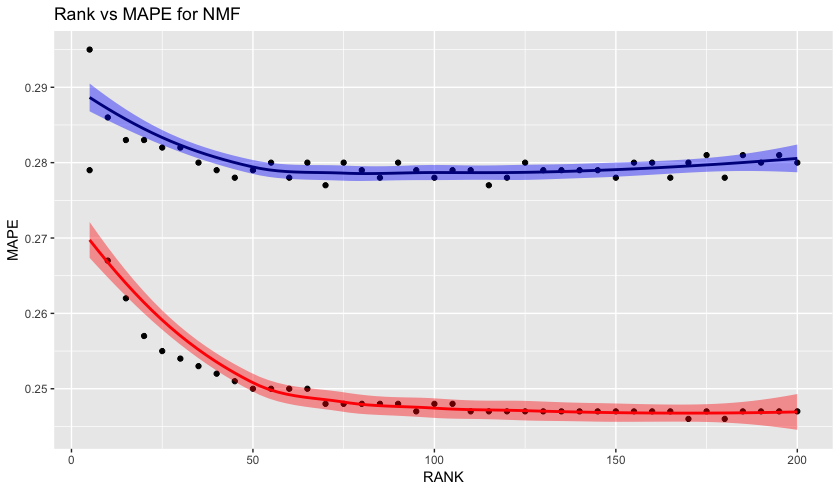
\includegraphics[scale=0.4]{RankVSMAPEforNNMF.png}

The blue curve represents the MAPE results for cross validation against the test set while the red curve represents the MAPE results for cross validation against the training set using the full data set. We can observe from the graph plotted that as rank increases, MAPE decreases, but increases slightly at the end, though the increase is small. We can roughly interpolate the U shape curve that we should expect. 

We can also observe that the MAPE values are generally lower in the red curve than in the blue curve. This is due to the fact that we used the same data set to train and test the model. We should be wary of being over-optimistic of such results as this may not be a good simulation of the prediction accuracy of the model in real life with other data sets. Perhaps the blue curve would be a better representation of the prediction accuracy of the model since the data set used to train the model is different from the data set used to test it. 

\end{document}